% !TeX program = xelatex
% !TeX encoding = UTF-8
% !TeX spellcheck = en_US
% !BIB program = biber
%% 
%% The above lines help editors like TeXstudio to automatically choose the right tools
%% to compile your LaTeX source file. If your tool does not support these magic comments,
%% you will need to make appropriate manual choices.
%% 
%% You can safely use "pdflatex" instead of "xelatex" if you prefer the pdfLaTeX toolchain.
%% However, pdfLaTeX will not be able to deliver the professional font experience that you
%% will get with XeLaTeX.
%% 
%% _Important_: These magic comments should be on the first lines of your source file.
%% 
%%%%%%%%%%%%%%%%%%%%%%%%%%%%%%%%%%%%%%%%%%%%%%%%%%%%%%%%%%%%%%%%%%%%%%%%%%%%%%%%

%%%%%%%%%%%%%%%%%%%%%%%%%%%%%%%%%%%%%%%%%%%%%%%%%%%%%%%%%%%%%%%%%%%%%%%%%%%%%%%%
%% 
%%            JJJJ   K                         K   UUUU         UUUU  
%%            JJJJ   KKKK                   KKKK   UUUU         UUUU  
%%            JJJJ   KKKKKK               KKKKKK   UUUU         UUUU  
%%            JJJJ      KKKKKK         KKKKKK      UUUU         UUUU  
%%            JJJJ         KKKKKK   KKKKKK         UUUU         UUUU  
%%            JJJJ            KKKKKKKKK            UUUU         UUUU  
%%    JJ     JJJJJ               KKK               UUUUU       UUUUU  
%%  JJJJJJJJJJJJJ    KKKKKKKKKKKKKKKKKKKKKKKKKKK    UUUUUUUUUUUUUUU   
%%    JJJJJJJJJ      KKKKKKKKKKKKKKKKKKKKKKKKKKK      UUUUUUUUUUU     
%% 
%% This is an example file for using the JKU LaTeX Beamer Theme.
%% 
%% Template created by Susanne Hametner and Doris Pargfrieder
%% Template altered by Pieter-Jan Hoedt (2020)
%% Template rewritten by Michael Roland (2021)
%% 
%%%%%%%%%%%%%%%%%%%%%%%%%%%%%%%%%%%%%%%%%%%%%%%%%%%%%%%%%%%%%%%%%%%%%%%%%%%%%%%%

%%%%%%%%%%%%%%%%%%%%%%%%%%%%%%%%%%%%%%%%%%%%%%%%%%%%%%%%%%%%%%%%%%%%%%%%%%%%%%%%
%% 
%% Document class: This is a LaTeX beamer presentation.
%% 
\documentclass[utf8,aspectratio=169,ngerman,english]{beamer}
%% 
%% The comma-separated list in square brackets are class options.
%% Useful options that you might want to use:
%% 
%% Define the aspect ratio of the slide layout:
%%  * aspectratio=169  ... 16:9 aspect ratio
%%  * aspectratio=43   ... 4:3 aspect ratio
%%  * aspectratio=1610 ... 16:10 aspect ratio
%% 
%% Define document languages:
%%  * ngerman ... German
%%  * english ... English
%%  * ...
%% 
%% Note that adding multiple document languages allows you to switch between these languages
%% within the document (using e.g. the `otherlanguage' environment). The last language in
%% the class options will be used as the default document language.
%% 
%% Switch to handout mode:
%%  * handout ... A compact mode that allows you to remove animation and skips slides for
%%                efficient printing.
%% 
%% Other options:
%%  * utf8 ... Treat input files as UTF-8 encoded. Make sure to always provide that option
%%             when you use pdfLaTeX so that pdfLaTeX knows how to read and interpret
%%             characters this source file.
%%  * c    ... Vertically center text on slides by default. You should avoid using this
%%             option. Only use this to restore the behavior of older versions of this theme.
%% 
%% _Important_: The document class should be the first line of LaTeX code in your main
%% source file. Do not place anything but comments / magic comments above that line (unless
%% you really know what you are doing).
%% 
%%%%%%%%%%%%%%%%%%%%%%%%%%%%%%%%%%%%%%%%%%%%%%%%%%%%%%%%%%%%%%%%%%%%%%%%%%%%%%%%

%%%%%%%%%%%%%%%%%%%%%%%%%%%%%%%%%%%%%%%%%%%%%%%%%%%%%%%%%%%%%%%%%%%%%%%%%%%%%%%%
%% 
%% Use the JKU LaTeX beamer theme for this presentation.
%% 
\usetheme[TNF,nosectionpage]{jku}
%\usetheme[darkmode,fancyfonts,totalframenumber,mathastext]{jku}
%% 
%% The comma-separated list in square brackets are theme options. Useful options that you
%% might want to use:
%% 
%% Color scheme selection options:
%%  * JKU  ... Use JKU (gray) color scheme (this is the default if no scheme is selected).
%%  * BUS  ... Use Business School color scheme.
%%  * LIT  ... Use Linz Institute of Technology color scheme.
%%  * MED  ... Use MED faculty color scheme.
%%  * RE   ... Use RE faculty color scheme.
%%  * SOE  ... Use School of Education color scheme.
%%  * SOWI ... Use SOWI faculty color scheme.
%%  * TNF  ... Use TNF faculty color scheme.
%% 
%% Color mode selection options:
%%  * darkmode ... Use dark color mode (where title and logo frames have a dark background).
%% 
%% Frame numbering options:
%%  * framenumber         ... Insert frame number into the frame footer.
%%  * totalframenumber    ... Insert frame number and total frame number into the frame footer
%%                            (only frames in the main part are counted).
%%  * appendixframenumber ... Similar to `totalframenumber', but count the overall total frame
%%                            number of main part and appendix.
%% 
%% Note that combining `totalframenumber' and `appendixframenumber' options will show the total
%% number of frames for the main part on frames in the main part and the overal total number of
%% frames for frames in the appendix.
%% 
%% Sectioning options:
%%  * nosectionpage       ... Supress section frames (see \section{<title>} command).
%%  * nosubsectionpage    ... Supress subsection frames (see \subsection{<title>} command).
%%  * nosubsubsectionpage ... Supress subsubsection frames (see \subsubsection{<title>} command).
%%  * partpage            ... Insert part frames (see \part{<title>} command).
%% 
%% Note that `nosectionpage' automatically sets `nosubsectionpage' and `nosubsubsectionpage'.
%% You could still e.g. show only subsubsection pages by using `nosectionpage,subsubsectionpage'.
%% 
%% Space-efficient monospace font options (requires XeTeX):
%%  * compactmono   ... Use condensed fixed-width font everywhere.
%%  * nocompactverb ... Do not use condensed fixed-width font for verbatim and listings.
%% 
%% Style-breaking options:
%%  * nojkufooter    ... Do not insert JKU/partner logos into the frame footer.
%%  * nofooter       ... Do not display a frame footer.
%%  * noimprint      ... Do not insert imprint on title pages.
%%  * frametitlecaps ... Set frame titles in capital letters (like in eariler theme versions).
%%  * nofancyfonts   ... Do not use custom TTF fonts with XeTeX / supress pdfLaTeX warning.
%%  * mac            ... Use adapted color palette for screen display on Mac.
%%  * legacyitemizestyle ... Use old bullet style in itemization.
%% 
%% Experimental options:
%%  * mathastext ... Use standard document fonts (and default to sans-serif font) in math mode
%% 
%% Advanced options:
%%  * nooptpackages     ... Do not load additional convenience packages (which are only there
%%                          to provide interoperability to the behavior of previous versions of
%%                          this theme but are not actually required for the current version).
%%  * logopath={<path>} ... Set the path where the theme can find its own logo resources. This
%%                          should typically be a relative path and the default is `./logos'.
%%  * fontpath={<path>} ... Set the path where the theme can find its own font resources. This
%%                          should typically be a relative path and the default is `./fonts'.
%% 
%% Hint: Boolean options can be used in the forms `option' or `option=true' the enable the
%% option and `nooption' or `option=false' to disable the option.
%% 
%%%%%%%%%%%%%%%%%%%%%%%%%%%%%%%%%%%%%%%%%%%%%%%%%%%%%%%%%%%%%%%%%%%%%%%%%%%%%%%%

%%%%%%%%%%%%%%%%%%%%%%%%%%%%%%%%%%%%%%%%%%%%%%%%%%%%%%%%%%%%%%%%%%%%%%%%%%%%%%%%
%% 
%% This is the place where you can load additional packages. If you want to load
%% a package `booktabs', you would use the command `\usepackage{booktabs}'.
%% 

\usepackage{booktabs}
\usepackage{tabularx}
%\usepackage{pifont}
%\newcommand{\cmark}{\ding{51}}
%\newcommand{\xmark}{\ding{55}}
%\newcommand{\rarr}{\ding{212}}
%\newcommand{\larr}{\raisebox{\depth}{\rotatebox{180}{\rarr}}}
\usepackage{csquotes}
\usepackage[backend=biber,citestyle=authoryear,sortcites=true,style=ACM-Reference-Format]{biblatex}

%% 
%%%%%%%%%%%%%%%%%%%%%%%%%%%%%%%%%%%%%%%%%%%%%%%%%%%%%%%%%%%%%%%%%%%%%%%%%%%%%%%%

%%%%%%%%%%%%%%%%%%%%%%%%%%%%%%%%%%%%%%%%%%%%%%%%%%%%%%%%%%%%%%%%%%%%%%%%%%%%%%%%
%% 
%% Set reasonable defaults for biblatex.
%% 

\preto{\bibsetup}{\providecommand*{\insertbiblabel}{}}
\DeclareFieldFormat*{title}{#1}
\DeclareFieldFormat*{booktitle}{#1}
\DeclareFieldFormat*{journaltitle}{#1}
\setcounter{biburlnumpenalty}{100}
\setcounter{biburllcpenalty}{100}
\setcounter{biburlucpenalty}{100}

%% Add bibligraphy source files
\addbibresource{references.bib}

%% 
%%%%%%%%%%%%%%%%%%%%%%%%%%%%%%%%%%%%%%%%%%%%%%%%%%%%%%%%%%%%%%%%%%%%%%%%%%%%%%%%


\begin{document}

%%%%%%%%%%%%%%%%%%%%%%%%%%%%%%%%%%%%%%%%%%%%%%%%%%%%%%%%%%%%%%%%%%%%%%%%%%%%%%%%
%% 
%% Presentation information and title page
%% 

%% Command \series{series title}: sets the series title
%\series{Space for your lecure title}

%% Command \title[short title]{title}: sets the presentation title
%% Command \titlesmall{text}: switches to small font size inside title
\title{Variations of the Eight Queens Puzzle}

%% Command \subtitle[short subtitle]{subtitle}: sets the presentation subtitle
%\subtitle{for \LaTeX\ Beamer}

%% Command \author[short authors]{authors}: sets the presentation authors (multiple authors may be separated with \and)
\author{Madhulika Mitra \and Jakob Weber \and David Auinger}

%% Command \institute{name}: sets the institute / author affiliation (style-breaking)
%\institute{Space for institute name}

%% Command \institutecode{CODE}: sets the institute abbreviation/initials (used to load the institute logo file, if present)
%\institutecode{INS}

%% Command \date[short date]{date}: sets the presentation date (short date is used in the footer by default)
%\date{\today}  % use this to set the date on the title page (style-breaking) and in the footer
\date[\today]{} % use this to set the date except for the title page (effectively in the footer only)

%% Command \partnerlogo[white=filename]{filename}: use filename as partner logo (leave filename blank to disable the partner logo), the optional argument ``white='' defines a separate file for use on dark background
%\partnerlogo{our_partner_logo}

%% Command \footer{text}: sets the footer field
%\footer{\insertshortsectiontitle} % the default
%\footer{\insertshorttitle}        % a good alternative

%% Command \footerdate{text}: sets the footer date field
%\footerdate{\insertshortdate} % the default

%% Command \footerpartnerlogo{filename}: use a different partner logo in the footer (e.g. a logo with a different form factor or no filename to disable the partner logo in the footer)
%\footerpartnerlogo{our_partner_logo}

%% Command \agenda[caption]{text}: sets the agenda (and optional caption) to display on the next title or section page
%\agenda[caption]{text}


%% Finally, print the title page using the above information:
%% 
%% \maketitle[options]
%%     Inserts a title page. The current standard faculty color theme and color
%%     mode are used by default, you may modify this using any of the following
%%     options:
%%      * light ... use light color theme
%%      * dark  ... use dark color theme
%%      * gray  ... use JKU gray color theme
%%      * black ... use black background
%%     In addition, options may contain a faculty name (see theme options) to
%%     use the faculty's color theme, e.g. `\maketitle[LIT,dark]'.
%% 
\maketitle
%% 
%% Note that you can even change the presentation information and print another
%% title page (with that updated information) ANYWHERE in your presentation.
%% 
%%%%%%%%%%%%%%%%%%%%%%%%%%%%%%%%%%%%%%%%%%%%%%%%%%%%%%%%%%%%%%%%%%%%%%%%%%%%%%%%


%% 
%% You can split your presentation into sections, subsections, and subsubsections,
%% just like you would do with any other LaTeX document. Depending on the chosen
%% theme options, frames showing the section titles will be inserted for each
%% sectioning command. You can use the starred versions of these commands (e.g.
%% `\section*{<title>}') to suppress specific section title frames.
%% 
\section{Introduction}

%% 
%% You create a new slide using the `frame' environment:
%% 
\begin{frame}
\frametitle{Introduction}

\begin{itemize}
\item The eight queens puzzle is a popular problem from 1848
\item A manifold of solutions and implementation already exists
\item Our goal is to solve a more general problem
\begin{itemize}
\item any rectangular board size
\item other types of pieces: knight, bishop, rook, queen, amazon
\item allow mixing different types
\end{itemize}
\end{itemize}
\end{frame}

\section{Approach and implementation}

\begin{frame}[containsverbatim]
\frametitle{Approach and implementation}
\begin{itemize}
\item Entry point \verb|main| function takes six lists as parameters
\begin{itemize}
\item board size (length and width)
\item five lists of pieces: knight, bishop, rook, queen, amazon
\item \verb|main([SizeX, SizeY], NS, BS, RS, QS, AS)|
\end{itemize}
\item Function \verb|possibleSolution| initializes all pieces
\item Function \verb|correctSolution| checks if initialization is a correct solution
\end{itemize}
\end{frame}

\begin{frame}
\frametitle{Challenges}
\begin{itemize}
\item Particular challenges due to mixing of types of pieces
\item Cannot assume that a piece not attacking another piece is not itself attacked
\begin{itemize}
\item Example: queen and knight, one might attack the other but not the other way
\item Need to check every piece against all other pieces of different types in both ways
\end{itemize}
\item Problems with permutations
\begin{itemize}
\item Prolog uses ordered lists, therefore permutations are considered unique solutions
\item However, this is not desired in our program
\item Define an order and only allow the permutation fulfilling the order
\end{itemize}
\end{itemize}
\end{frame}

\begin{frame}
\frametitle{Pieces in detail}
\begin{itemize}
\item Essentially two possibilities of attacks
\begin{itemize}
\item moving to defined locations relative to current location (knight)
\item moving arbitrary distance in certain direction (bishop, rook, queen)
\end{itemize}
\item Solve the knight by checking each knight with every other piece
\begin{itemize}
\item no other piece in same location
\item no other piece in any of the eight locations possibly attacked by knight
\item use recursion to apply checks to all pieces
\end{itemize}
\item Solve the bishop with similar recursion but different check
\begin{itemize}
\item no other piece in same diagonals
\end{itemize}
\item Similar checks for rook and queen
\item Solve amazon by combining the checks of the knight and queen
\end{itemize}
\end{frame}

\section{Usage}

\begin{frame}[containsverbatim]
\frametitle{Usage}
\begin{itemize}
\item Input
\begin{itemize}
\item classic eight queens puzzle \\
\verb|main([8, 8], [], [], [], [Q1, Q2, Q3, Q4, Q5, Q6, Q7, Q8], []).|
\item all types once on 5x5 board \\
\verb|main([5,5],[N],[B],[R],[Q],[A]).|
\end{itemize}
\item Output prints locations of input pieces for a solution
\item Also possible to count all solutions \\
\verb|countSolutions([8, 8], [], [], [], [Q1, Q2, Q3, Q4, Q5, Q6, Q7, Q8], []).|
\end{itemize}
\end{frame}

\section{Examples}

\begin{frame}[containsverbatim]
\frametitle{Classic eight queens problem}
\makebox[0pt][l]{
  \raisebox{-5.5cm}[0pt][0pt]{
    \hspace*{7cm}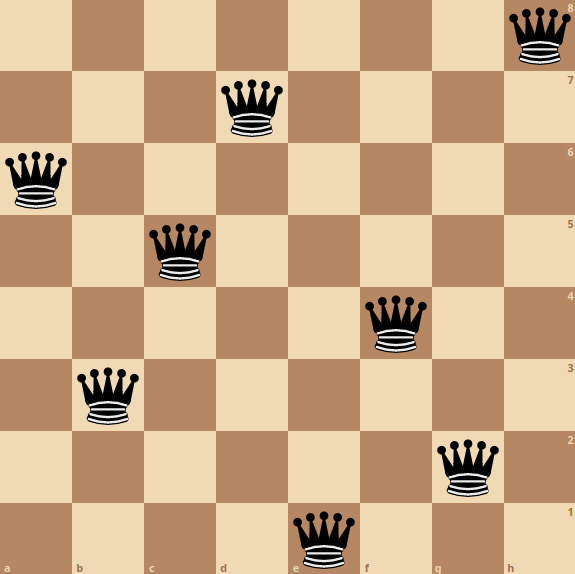
\includegraphics[width=4cm]{images/8queens.png}}}
\begin{verbatim}
?- main([8, 8], [], [], [], [Q1, Q2, Q3, Q4, Q5, Q6, Q7, Q8], []).
Q1 = [1, 4],
Q2 = [2, 2],
Q3 = [3, 7],
Q4 = [4, 3],
Q5 = [5, 6],
Q6 = [6, 8],
Q7 = [7, 5],
Q8 = [8, 1]
\end{verbatim}
\end{frame}

\begin{frame}[containsverbatim]
\frametitle{All types once}
\makebox[0pt][l]{
  \raisebox{-5.5cm}[0pt][0pt]{
    \hspace*{7cm}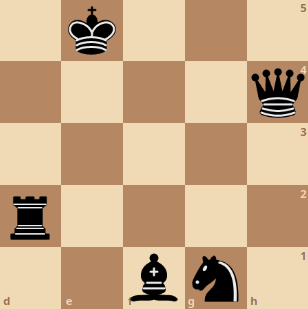
\includegraphics[width=4cm]{images/prolog_mixed_solution.png}}}
\begin{verbatim}
?- main([5,5],[N],[B],[R],[Q],[A]).
N = [1, 2],
B = [1, 3],
R = [2, 5],
Q = [4, 1],
A = [5, 4]
\end{verbatim}
\end{frame}

\section{Conclusion}

\begin{frame}
\frametitle{Conclusion}
\begin{itemize}
\item Successfully solves already solved problems
\item Generalizes to different board sizes, other pieces, mixing of pieces
\item Multitude of new problems and experiments possible
\end{itemize}
\end{frame}

\jkulogo

\end{document}
\endinput
